% Options for packages loaded elsewhere
\PassOptionsToPackage{unicode}{hyperref}
\PassOptionsToPackage{hyphens}{url}
%
\documentclass[
]{book}
\usepackage{amsmath,amssymb}
\usepackage{lmodern}
\usepackage{iftex}
\ifPDFTeX
  \usepackage[T1]{fontenc}
  \usepackage[utf8]{inputenc}
  \usepackage{textcomp} % provide euro and other symbols
\else % if luatex or xetex
  \usepackage{unicode-math}
  \defaultfontfeatures{Scale=MatchLowercase}
  \defaultfontfeatures[\rmfamily]{Ligatures=TeX,Scale=1}
\fi
% Use upquote if available, for straight quotes in verbatim environments
\IfFileExists{upquote.sty}{\usepackage{upquote}}{}
\IfFileExists{microtype.sty}{% use microtype if available
  \usepackage[]{microtype}
  \UseMicrotypeSet[protrusion]{basicmath} % disable protrusion for tt fonts
}{}
\makeatletter
\@ifundefined{KOMAClassName}{% if non-KOMA class
  \IfFileExists{parskip.sty}{%
    \usepackage{parskip}
  }{% else
    \setlength{\parindent}{0pt}
    \setlength{\parskip}{6pt plus 2pt minus 1pt}}
}{% if KOMA class
  \KOMAoptions{parskip=half}}
\makeatother
\usepackage{xcolor}
\IfFileExists{xurl.sty}{\usepackage{xurl}}{} % add URL line breaks if available
\IfFileExists{bookmark.sty}{\usepackage{bookmark}}{\usepackage{hyperref}}
\hypersetup{
  pdftitle={SCMA469 Actuarial Statistics},
  pdfauthor={Pairote Satiracoo},
  hidelinks,
  pdfcreator={LaTeX via pandoc}}
\urlstyle{same} % disable monospaced font for URLs
\usepackage[margin=1in]{geometry}
\usepackage{color}
\usepackage{fancyvrb}
\newcommand{\VerbBar}{|}
\newcommand{\VERB}{\Verb[commandchars=\\\{\}]}
\DefineVerbatimEnvironment{Highlighting}{Verbatim}{commandchars=\\\{\}}
% Add ',fontsize=\small' for more characters per line
\usepackage{framed}
\definecolor{shadecolor}{RGB}{248,248,248}
\newenvironment{Shaded}{\begin{snugshade}}{\end{snugshade}}
\newcommand{\AlertTok}[1]{\textcolor[rgb]{0.94,0.16,0.16}{#1}}
\newcommand{\AnnotationTok}[1]{\textcolor[rgb]{0.56,0.35,0.01}{\textbf{\textit{#1}}}}
\newcommand{\AttributeTok}[1]{\textcolor[rgb]{0.77,0.63,0.00}{#1}}
\newcommand{\BaseNTok}[1]{\textcolor[rgb]{0.00,0.00,0.81}{#1}}
\newcommand{\BuiltInTok}[1]{#1}
\newcommand{\CharTok}[1]{\textcolor[rgb]{0.31,0.60,0.02}{#1}}
\newcommand{\CommentTok}[1]{\textcolor[rgb]{0.56,0.35,0.01}{\textit{#1}}}
\newcommand{\CommentVarTok}[1]{\textcolor[rgb]{0.56,0.35,0.01}{\textbf{\textit{#1}}}}
\newcommand{\ConstantTok}[1]{\textcolor[rgb]{0.00,0.00,0.00}{#1}}
\newcommand{\ControlFlowTok}[1]{\textcolor[rgb]{0.13,0.29,0.53}{\textbf{#1}}}
\newcommand{\DataTypeTok}[1]{\textcolor[rgb]{0.13,0.29,0.53}{#1}}
\newcommand{\DecValTok}[1]{\textcolor[rgb]{0.00,0.00,0.81}{#1}}
\newcommand{\DocumentationTok}[1]{\textcolor[rgb]{0.56,0.35,0.01}{\textbf{\textit{#1}}}}
\newcommand{\ErrorTok}[1]{\textcolor[rgb]{0.64,0.00,0.00}{\textbf{#1}}}
\newcommand{\ExtensionTok}[1]{#1}
\newcommand{\FloatTok}[1]{\textcolor[rgb]{0.00,0.00,0.81}{#1}}
\newcommand{\FunctionTok}[1]{\textcolor[rgb]{0.00,0.00,0.00}{#1}}
\newcommand{\ImportTok}[1]{#1}
\newcommand{\InformationTok}[1]{\textcolor[rgb]{0.56,0.35,0.01}{\textbf{\textit{#1}}}}
\newcommand{\KeywordTok}[1]{\textcolor[rgb]{0.13,0.29,0.53}{\textbf{#1}}}
\newcommand{\NormalTok}[1]{#1}
\newcommand{\OperatorTok}[1]{\textcolor[rgb]{0.81,0.36,0.00}{\textbf{#1}}}
\newcommand{\OtherTok}[1]{\textcolor[rgb]{0.56,0.35,0.01}{#1}}
\newcommand{\PreprocessorTok}[1]{\textcolor[rgb]{0.56,0.35,0.01}{\textit{#1}}}
\newcommand{\RegionMarkerTok}[1]{#1}
\newcommand{\SpecialCharTok}[1]{\textcolor[rgb]{0.00,0.00,0.00}{#1}}
\newcommand{\SpecialStringTok}[1]{\textcolor[rgb]{0.31,0.60,0.02}{#1}}
\newcommand{\StringTok}[1]{\textcolor[rgb]{0.31,0.60,0.02}{#1}}
\newcommand{\VariableTok}[1]{\textcolor[rgb]{0.00,0.00,0.00}{#1}}
\newcommand{\VerbatimStringTok}[1]{\textcolor[rgb]{0.31,0.60,0.02}{#1}}
\newcommand{\WarningTok}[1]{\textcolor[rgb]{0.56,0.35,0.01}{\textbf{\textit{#1}}}}
\usepackage{longtable,booktabs,array}
\usepackage{calc} % for calculating minipage widths
% Correct order of tables after \paragraph or \subparagraph
\usepackage{etoolbox}
\makeatletter
\patchcmd\longtable{\par}{\if@noskipsec\mbox{}\fi\par}{}{}
\makeatother
% Allow footnotes in longtable head/foot
\IfFileExists{footnotehyper.sty}{\usepackage{footnotehyper}}{\usepackage{footnote}}
\makesavenoteenv{longtable}
\usepackage{graphicx}
\makeatletter
\def\maxwidth{\ifdim\Gin@nat@width>\linewidth\linewidth\else\Gin@nat@width\fi}
\def\maxheight{\ifdim\Gin@nat@height>\textheight\textheight\else\Gin@nat@height\fi}
\makeatother
% Scale images if necessary, so that they will not overflow the page
% margins by default, and it is still possible to overwrite the defaults
% using explicit options in \includegraphics[width, height, ...]{}
\setkeys{Gin}{width=\maxwidth,height=\maxheight,keepaspectratio}
% Set default figure placement to htbp
\makeatletter
\def\fps@figure{htbp}
\makeatother
\setlength{\emergencystretch}{3em} % prevent overfull lines
\providecommand{\tightlist}{%
  \setlength{\itemsep}{0pt}\setlength{\parskip}{0pt}}
\setcounter{secnumdepth}{5}
\usepackage{booktabs}
\usepackage{amsthm}
\usepackage{LectureNoteMacro}
\makeatletter
\def\thm@space@setup{%
  \thm@preskip=8pt plus 2pt minus 4pt
  \thm@postskip=\thm@preskip
}
\makeatother
\ifLuaTeX
  \usepackage{selnolig}  % disable illegal ligatures
\fi
\usepackage[]{natbib}
\bibliographystyle{apalike}

\title{SCMA469 Actuarial Statistics}
\author{Pairote Satiracoo}
\date{2021-08-08}

\usepackage{amsthm}
\newtheorem{theorem}{Theorem}[chapter]
\newtheorem{lemma}{Lemma}[chapter]
\newtheorem{corollary}{Corollary}[chapter]
\newtheorem{proposition}{Proposition}[chapter]
\newtheorem{conjecture}{Conjecture}[chapter]
\theoremstyle{definition}
\newtheorem{definition}{Definition}[chapter]
\theoremstyle{definition}
\newtheorem{example}{Example}[chapter]
\theoremstyle{definition}
\newtheorem{exercise}{Exercise}[chapter]
\theoremstyle{definition}
\newtheorem{hypothesis}{Hypothesis}[chapter]
\theoremstyle{remark}
\newtheorem*{remark}{Remark}
\newtheorem*{solution}{Solution}
\begin{document}
\maketitle

{
\setcounter{tocdepth}{1}
\tableofcontents
}
\hypertarget{prerequisites}{%
\chapter{Prerequisites}\label{prerequisites}}

This is a \emph{sample} book written in \textbf{Markdown}. You can use anything that Pandoc's Markdown supports, e.g., a math equation \(a^2 + b^2 = c^2\).

The \textbf{bookdown} package can be installed from CRAN or Github:

\begin{Shaded}
\begin{Highlighting}[]
\FunctionTok{install.packages}\NormalTok{(}\StringTok{"bookdown"}\NormalTok{)}
\CommentTok{\# or the development version}
\CommentTok{\# devtools::install\_github("rstudio/bookdown")}
\end{Highlighting}
\end{Shaded}

Remember each Rmd file contains one and only one chapter, and a chapter is defined by the first-level heading \texttt{\#}.

To compile this example to PDF, you need XeLaTeX. You are recommended to install TinyTeX (which includes XeLaTeX): \url{https://yihui.name/tinytex/}.

\hypertarget{intro}{%
\chapter{Introduction to Stochastic Processes}\label{intro}}

You can label chapter and section titles using \texttt{\{\#label\}} after them, e.g., we can reference Chapter \ref{intro}. If you do not manually label them, there will be automatic labels anyway, e.g., Chapter \ref{methods}.

Figures and tables with captions will be placed in \texttt{figure} and \texttt{table} environments, respectively.

\begin{Shaded}
\begin{Highlighting}[]
\FunctionTok{par}\NormalTok{(}\AttributeTok{mar =} \FunctionTok{c}\NormalTok{(}\DecValTok{4}\NormalTok{, }\DecValTok{4}\NormalTok{, .}\DecValTok{1}\NormalTok{, .}\DecValTok{1}\NormalTok{))}
\FunctionTok{plot}\NormalTok{(pressure, }\AttributeTok{type =} \StringTok{\textquotesingle{}b\textquotesingle{}}\NormalTok{, }\AttributeTok{pch =} \DecValTok{19}\NormalTok{)}
\end{Highlighting}
\end{Shaded}

\begin{figure}

{\centering 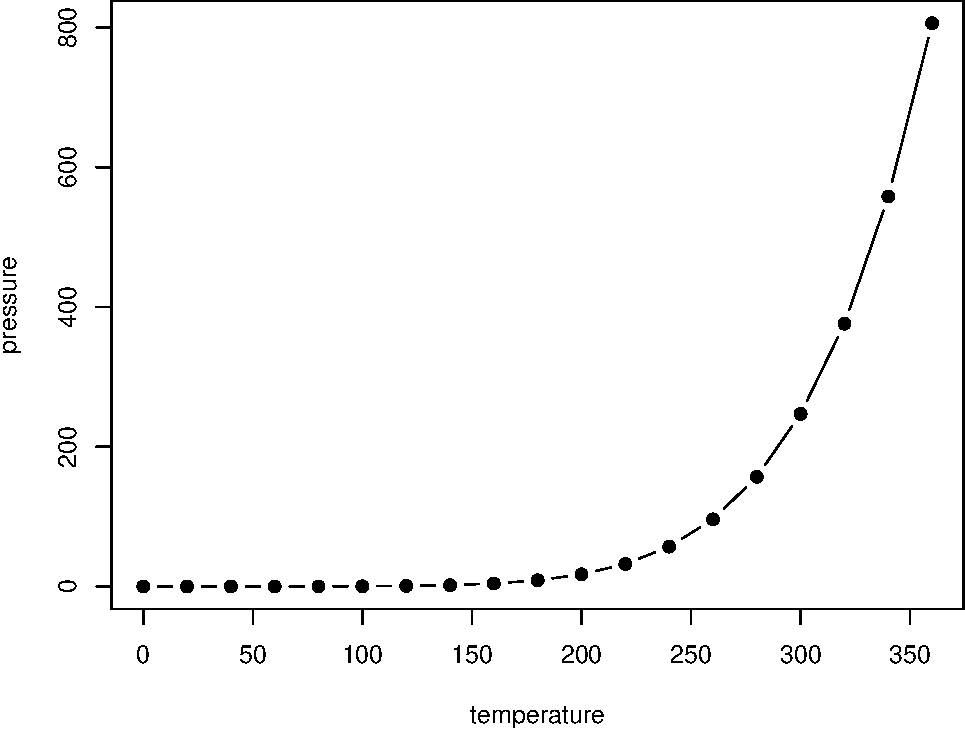
\includegraphics[width=0.8\linewidth]{bookdownproj_files/figure-latex/nice-fig-1} 

}

\caption{Here is a nice figure!}\label{fig:nice-fig}
\end{figure}

Reference a figure by its code chunk label with the \texttt{fig:} prefix, e.g., see Figure \ref{fig:nice-fig}. Similarly, you can reference tables generated from \texttt{knitr::kable()}, e.g., see Table \ref{tab:nice-tab}.

\begin{Shaded}
\begin{Highlighting}[]
\NormalTok{knitr}\SpecialCharTok{::}\FunctionTok{kable}\NormalTok{(}
  \FunctionTok{head}\NormalTok{(iris, }\DecValTok{20}\NormalTok{), }\AttributeTok{caption =} \StringTok{\textquotesingle{}Here is a nice table!\textquotesingle{}}\NormalTok{,}
  \AttributeTok{booktabs =} \ConstantTok{TRUE}
\NormalTok{)}
\end{Highlighting}
\end{Shaded}

\begin{table}

\caption{\label{tab:nice-tab}Here is a nice table!}
\centering
\begin{tabular}[t]{rrrrl}
\toprule
Sepal.Length & Sepal.Width & Petal.Length & Petal.Width & Species\\
\midrule
5.1 & 3.5 & 1.4 & 0.2 & setosa\\
4.9 & 3.0 & 1.4 & 0.2 & setosa\\
4.7 & 3.2 & 1.3 & 0.2 & setosa\\
4.6 & 3.1 & 1.5 & 0.2 & setosa\\
5.0 & 3.6 & 1.4 & 0.2 & setosa\\
\addlinespace
5.4 & 3.9 & 1.7 & 0.4 & setosa\\
4.6 & 3.4 & 1.4 & 0.3 & setosa\\
5.0 & 3.4 & 1.5 & 0.2 & setosa\\
4.4 & 2.9 & 1.4 & 0.2 & setosa\\
4.9 & 3.1 & 1.5 & 0.1 & setosa\\
\addlinespace
5.4 & 3.7 & 1.5 & 0.2 & setosa\\
4.8 & 3.4 & 1.6 & 0.2 & setosa\\
4.8 & 3.0 & 1.4 & 0.1 & setosa\\
4.3 & 3.0 & 1.1 & 0.1 & setosa\\
5.8 & 4.0 & 1.2 & 0.2 & setosa\\
\addlinespace
5.7 & 4.4 & 1.5 & 0.4 & setosa\\
5.4 & 3.9 & 1.3 & 0.4 & setosa\\
5.1 & 3.5 & 1.4 & 0.3 & setosa\\
5.7 & 3.8 & 1.7 & 0.3 & setosa\\
5.1 & 3.8 & 1.5 & 0.3 & setosa\\
\bottomrule
\end{tabular}
\end{table}

You can write citations, too. For example, we are using the \textbf{bookdown} package \citep{R-bookdown} in this sample book, which was built on top of R Markdown and \textbf{knitr} \citep{xie2015}.

The course will cover the probabilistic framework for stochastic models
of real-world applications with emphasis on actuarial work. We will
illustrate some practical actuarial problems for which we will develop
mathematical models, tools and techniques for analysing and quantifying
the uncertainty of the problems.

Here are some of the examples which will be covered later in the course.

\hypertarget{examples-of-real-world-processes}{%
\chapter{Examples of real world processes}\label{examples-of-real-world-processes}}

\begin{example}
\protect\hypertarget{exm:unlabeled-div-1}{}\label{exm:unlabeled-div-1}

\textbf{Example 1}. \emph{(\textbf{No claims discount systems (NCD)}) A well-known
model widely used by auto insurance companies is the \textbf{no claims
discount system}, in which an insured receives a discount for a claim
free year, while the insured is penalised by an additional premium when
one or more accidents occur.}

\emph{An example of the NCD system in UK may be structured as follows:}

\begin{longtable}[]{@{}cccccccc@{}}
\toprule
\emph{Level} & \emph{7} & \emph{6} & \emph{5} & \emph{4} & \emph{3} & \emph{2} & \emph{1} \\
\midrule
\endhead
\emph{Premium} & \emph{100\%} & \emph{75\%} & \emph{65\%} & \emph{55\%} & \emph{45\%} & \emph{40\%} & \emph{33\%} \\
\bottomrule
\end{longtable}

\emph{The rules for moving between these levels are as follows:}

\begin{itemize}
\item
  \emph{For a claim-free year, a policyholder moves down 1 level.}
\item
  \emph{Levels 4\$-\$7:}

  \begin{itemize}
  \item
    \emph{For every one claim, the policyholder moves up 1 level or
    remains at level 7.}
  \item
    \emph{For every two or more claims, move to, or remains at, level 7.}
  \end{itemize}
\item
  \emph{Levels 2\$-\$3:}

  \begin{itemize}
  \item
    \emph{For every one claim, move up 2 levels.}
  \item
    \emph{For every two claims, move up 4 levels.}
  \item
    \emph{For every three or more claims, move to level 7.}
  \end{itemize}
\item
  \emph{Level 1:}

  \begin{itemize}
  \item
    \emph{For every one claim, move to level 4.}
  \item
    \emph{For every two claims, move to level 6.}
  \item
    \emph{For every three or more claims, move to level 7.}
  \end{itemize}
\end{itemize}

\emph{The no claims discount system is a form of experience rating consisting
of a finite number of levels (or classes), each with its own premium.
The 7 levels are experience-rated as described above.}

\emph{For the NCD model, questions of interest may include:}

\begin{enumerate}
\def\labelenumi{\arabic{enumi}.}
\item
  \emph{For 10,000 policyholders at level 7, estimate the }expected
  numbers* at each discount level at a given time, or once stability
  has been achieved.*
\item
  \emph{What is the }probability* that a policyholder who is at a specific
  discount level (i.e.~one of the levels 1-6) has no discount after 2
  years?*
\item
  \emph{What is the }distribution* of being in one of the levels at time 5
  years?*
\item
  \emph{Suppose a large number of people having the same claim
  probabilities take out policies at the same time. What is the
  proportion would you expect to be in each discount level in the long
  run?}
\end{enumerate}

\emph{What would be a suitable model to study the NCD system? As opposed to a
\textbf{deterministic model} for which its outcomes are fixed, the outcomes
of the NCD model are uncertain. It turns out that the NCD system can be
studied within the framework of Markov chains, which are examples of
stochastic processes. The use of matrix algebra provides a powerful tool
to understand and analyse the processes.}

\emph{The evolution of the states or levels can be described the random
variables \(X_0, X_1,X_2, \ldots\) and probability distributions, where
\(X_n\) is the level of the policyholder at time \(n\). In this example, the
set of all states called the state space is discrete, which consists of
seven levels, and the time variable is also discrete. This is an example
of a \textbf{discrete time, discrete state space stochastic process}.}

\end{example}

\begin{example}
\protect\hypertarget{exm:unlabeled-div-2}{}\label{exm:unlabeled-div-2}

\textbf{Example 2}. \emph{(\textbf{Poisson processes}) Consider the number of claims
that occur up to time \(t\) (denoted by \(N_t\)) from a portfolio of health
insurance policies (or other types of insurance products). Suppose that
the average rate of occurrence of claims per time unit (e.g.~day or week
) is given by \(\lambda\).}

\emph{Here are some questions of interest:}

\begin{enumerate}
\def\labelenumi{\arabic{enumi}.}
\item
  \emph{On average, 20 claims arrive every day, what is the probability
  that more than 100 claims arrive within a week?}
\item
  \emph{What is the expected time until the next claim?}
\end{enumerate}

\emph{In this example, the state space consists of all whole numbers
\(\{0, 1, 2, \ldots\}\), while the time variable is continuous. The
process is a \textbf{continuous-time stochastic process with discrete state
space}. The model used to model the insurance claims is an example of
\textbf{Poisson processes}. The Poisson process is one of the most
widely-used counting processes. Even thought we know that claims occur
at a certain rate, but completely at random. Moreover, the timing
between claims seem to be completely random.}

\emph{Later, we will see that there are several ways to describe this
process. One can focus on the number of claims that occur up to time \(t\)
or the times between those claims when they occur. Many important
properties of Poisson processes will be discussed.}

\end{example}

\begin{example}
\protect\hypertarget{exm:unlabeled-div-3}{}\label{exm:unlabeled-div-3}

\textbf{Example 3}. \emph{(\textbf{Markov processes}) Suppose that we observe a total
of \(n\) independent lives all aged between \(x\) and \(x + 1\). For life \(i\),
we define the following terms:}

\begin{itemize}
\item
  \emph{\(x+ a_i\) is the age at which observation
  begins,\(\quad 0 \le a_i < 1\).}
\item
  \emph{\(x+ b_i\) is the age at which observation ends, if life does not
  die, \(\quad 0 \le b_i < 1\).}
\item
  \emph{\(x+ t_i\) is the age at which observation stops, by death or
  censoring.}
\item
  \emph{\(d_i = 1\), if life \(i\) dies, otherwise \(d_i = 0\), if life \(i\)
  censored.}
\end{itemize}

\emph{For example, consider the following mortality data on eight lives all
aged between \(70\) and \(71\).}

\begin{longtable}[]{@{}ccccc@{}}
\toprule
\emph{Life} & \emph{\(a_i\)} & \emph{\(b_i\)} & \emph{\(d_i\)} & \emph{\(t_i\)} \\
\midrule
\endhead
\emph{1} & \emph{0} & \emph{1} & \emph{1} & \emph{0.25} \\
\emph{2} & \emph{0} & \emph{1} & \emph{1} & \emph{0.75} \\
\emph{3} & \emph{0} & \emph{1} & \emph{0} & \emph{1} \\
\emph{4} & \emph{0.1} & \emph{0.6} & \emph{1} & \emph{0.5} \\
\emph{5} & \emph{0.2} & \emph{0.7} & \emph{1} & \emph{0.6} \\
\emph{6} & \emph{0.2} & \emph{0.4} & \emph{0} & \emph{0.4} \\
\emph{7} & \emph{0.5} & \emph{1} & \emph{1} & \emph{0.75} \\
\emph{8} & \emph{0.5} & \emph{0.75} & \emph{0} & \emph{0.75} \\
\bottomrule
\end{longtable}

\emph{How would one use this dataset to estimate the probability that a life
aged 70 dies before age \(70 + t\) or survives to at least age \(70 + t\),
for \(t \in [0,1)\)?}

\emph{In this example, we can represent the process by \(\{X_t\}_{t \ge 0}\)
with two possible states (alive or dead). This model is also an example
of a \textbf{continuous-time stochastic process with discrete state space}.}

\emph{Here, we illustrate three actuarial applications which can be modelled
by some \textbf{stochastic processes}. We should also emphasis that the
outcome of one of the above processes is not fixed or uncertain. The
course will provide important tools and techniques to analyse the
problems with the goal of quantifying the uncertainty in the system.}

\end{example}

\hypertarget{discrete-time-markov-chains}{%
\chapter{Discrete-time Markov chains}\label{discrete-time-markov-chains}}

--\textgreater{}

--\textgreater{}

\hypertarget{methods}{%
\chapter{Methods}\label{methods}}

We describe our methods in this chapter.

Math can be added in body using usual syntax like this

\hypertarget{math-example}{%
\section{math example}\label{math-example}}

\(p\) is unknown but expected to be around 1/3. Standard error will be approximated

\[
SE = \sqrt(\frac{p(1-p)}{n}) \approx \sqrt{\frac{1/3 (1 - 1/3)} {300}} = 0.027
\]

You can also use math in footnotes like this\footnote{where we mention \(p = \frac{a}{b}\)}.

We will approximate standard error to 0.027\footnote{\(p\) is unknown but expected to be around 1/3. Standard error will be approximated

  \[
  SE = \sqrt(\frac{p(1-p)}{n}) \approx \sqrt{\frac{1/3 (1 - 1/3)} {300}} = 0.027
  \]}

\hypertarget{applications}{%
\chapter{Applications}\label{applications}}

Some \emph{significant} applications are demonstrated in this chapter.

\hypertarget{datacamp-light}{%
\section{DataCamp Light}\label{datacamp-light}}

By default, \texttt{tutorial} will convert all R chunks.

eyJsYW5ndWFnZSI6InIiLCJzYW1wbGUiOiJhIDwtIDJcbmIgPC0gM1xuXG5hICsgYiJ9

\hypertarget{final-words}{%
\chapter{Final Words}\label{final-words}}

We have finished a nice book.

  \bibliography{book.bib,packages.bib}

\end{document}
